\chapter{Introduction} \label{ch: introduction}

\graphicspath{{01-introduction/figures/}}

\begin{chapterquote}[Lewis Carroll][Alice in Wonderland][Chapter XII]
  ``Begin at the beginning,'' the King said, very gravely,
  ``and go on till you come to the end: then stop.
\end{chapterquote}

In this introductory Chapter we briefly introduce the field of solar physics and elaborate a bit further on the outer layers of the sun itself. Some general terminology will be introduced while also discussing certain features observable in the solar atmosphere, since they are quite relevant in the scope of early Chapters. Eventually we bring waves and instabilities into play, as they are in essence a main topic in this thesis, and discuss their importance both in a solar physical context as well as in more general (astro)physical settings.

\section{A very brief history of astrophysics}
The wonderful field of astrophysics encompasses a plethora of different disciplines. Historically, astrophysics has its roots in astronomy, which is in itself a millennia-old science. Back in ancient Greece people were already wondering about various heavenly objects and how to explain their peculiar motions, and centuries later it was realised that these objects actually obey natural laws. Since then the field of astrophysics has greatly expanded, including not only observational astronomy, but also computational and theoretical astrophysics, quantum mechanics, nuclear physics and even chemistry; and the list has recently been expanded even further, now also including gravitational wave astronomy. All these fields are intricately linked, depending on the objects that are being studied. While historically astronomy ``only'' studied the motions of stars and planets, we now know that there are a myriad of fascinating objects all around us: stars actually exist in all sorts and sizes, depending on how far along they are in their evolutionary process; ranging from huge supergiants to regular sized stars such as the sun, to baby proto-stars that are not even ``born'' yet. The list can be further extended with planetary systems, nebulae, and more exotic objects such as neutron stars or black holes, with the latter typically being accompanied with high-energy jets.

\begin{figure}[t]
  \centering
  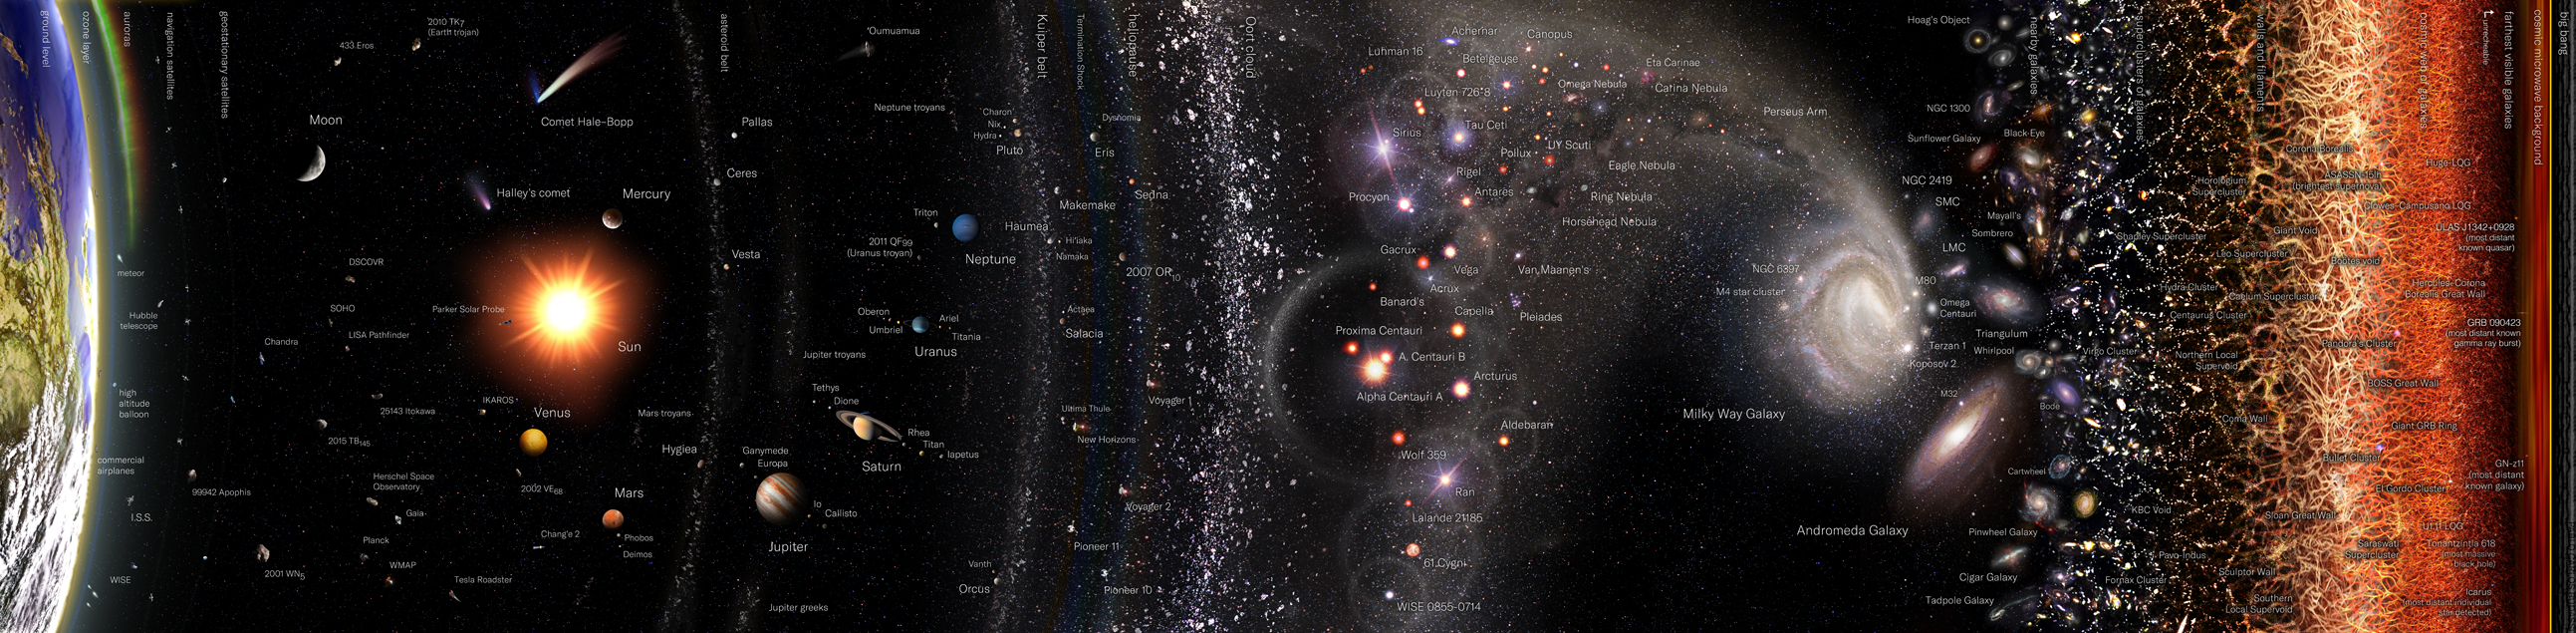
\includegraphics[width=\textwidth]{observable_universe.png}
  \caption{
    Artistic rendering of the observable universe, shown on a logarithmic scale from left to right based on proximity to Earth. Figure by Pablo Carlos Budassi.
  }
\end{figure}

In most (if not all) fields related to astrophysics research deals with \emph{plasma}, as it is by far the most abundant form of ordinary matter in the universe (we say ``ordinary'' here as we explicitly exclude exotic stuff such as dark matter and dark energy). A plasma can be simplified as an ionised gas, hence a significant part of it are charged particles which in turn implies that electromagnetic fields are of extreme importance. Depending on the amount of neutral particles present a plasma can either be fully ionised (no neutrals) or partially ionised (some neutrals). In this thesis we only consider a fully ionised plasma, which will be quite sufficient for (most of) our applications.

The tools used to study astrophysics vary greatly, and similar to the various disciplines depend on which objects are being studied. In the time of Newton and Galilei tools mostly consisted of early telescopes and basic mathematical methods. Over the years new theories have been developed, where Einstein's general relativity is probably the most notable in an astrophysical context, which came accompanied with numerous advances and physical insights. From an observational viewpoint we evolved from using basic, simple telescopes to (arrays of) huge ground and space based telescopes and observatories designed to probe the deepest reaches of our universe. Additionally, with the advent of the computer age a completely new set of tools became available: suddenly it was possible to numerically solve systems of equations that were previously unsolvable using analytical methods, and this in turn sparked a whole new branch of computational astrophysics. Large-scale numerical codes have been developed since then, which can exploit a huge number of computational resources in parallel using the most powerful supercomputers on the planet. This has opened a completely new door into the wonderful world of astrophysics, where it is now possible to numerically probe and visualise even the most exotic astrophysical objects at extreme resolutions.

The field of solar physics studies, as the name suggests, our sun. Even here research topics are widely spread out, ranging from the solar interior to features on the solar surface, to the entire solar atmosphere, the link between the solar wind and space weather, to name a few. In this thesis we will mainly focus on waves and instability aspects from a spectroscopic standpoint, which can be directly linked to interesting structures in the solar atmosphere, that is, parts of the solar corona and chromosphere. We will mainly rely on numerical approaches, supplemented with a strong mathematical foundation.


\section{The Sun in a nutshell}
Our sun, at a distance of approximately 150 million kilometres, is the closest star to Earth and is directly responsible for all life on this planet. Roughly five billion years ago a ``baby'' sun (or proto-star) formed as a contracting molecular cloud, slowly heating up in the process. Once the proto-star's core temperature became high enough nuclear fusion kicked in, converting hydrogen to helium. This signalled a delicate balance between inwards gravitational forces and the outwards push of energy in the form of luminosity, contraction ceased, and our sun entered its main sequence phase as a standard G-type main sequence star. Since then it has been happily burning hydrogen and turning it to helium in its core, and will continue to do so for roughly another 5 billion years. At that point all hydrogen in the core will be exhausted and the star will expand into a red giant, eventually turning into a white dwarf.

The sun is essentially a giant ball of plasma with various internal regions having different physical properties. We will not discuss the overall structure of the solar interior here, but focus only on the solar atmosphere. The sun does not have a strict ``surface'', in the sense that there is no abrupt border between the atmosphere and interior like we have here on Earth; it rather is defined as the part of the sun where photons can easily escape into space. This is marked by an optical depth of $\tau_\nu \approx 1$, which is a measure of how a given intensity is absorbed when it passes through a certain layer, in essence the transparency of this layer. The solar interior has an optical depth which is much larger than one, whereas the solar exterior has an optical depth much less than one, and can (for the most part) be considered to be optically thin. For an extensive discussion on the properties of the solar interior and exterior, see \citet{book_priest}.

Figure \ref{fig: solar_profile} shows a sketch of the solar atmosphere, which can be divided into three separate regions. While in reality the entire atmosphere is highly dynamic and varying in time, for all intents and purposes we can conveniently model it as three layers with different properties. The first one is called the \emph{photosphere}, which is a thin layer only a few 100 kms thick emitting most of the sun's visible light. It is pervaded with granulation of different sizes, owing their existence to convective cells originating from within the solar interior, implying that there is quite a lot of turbulence present throughout the entire solar photosphere.
\begin{figure}[t]
  \centering
  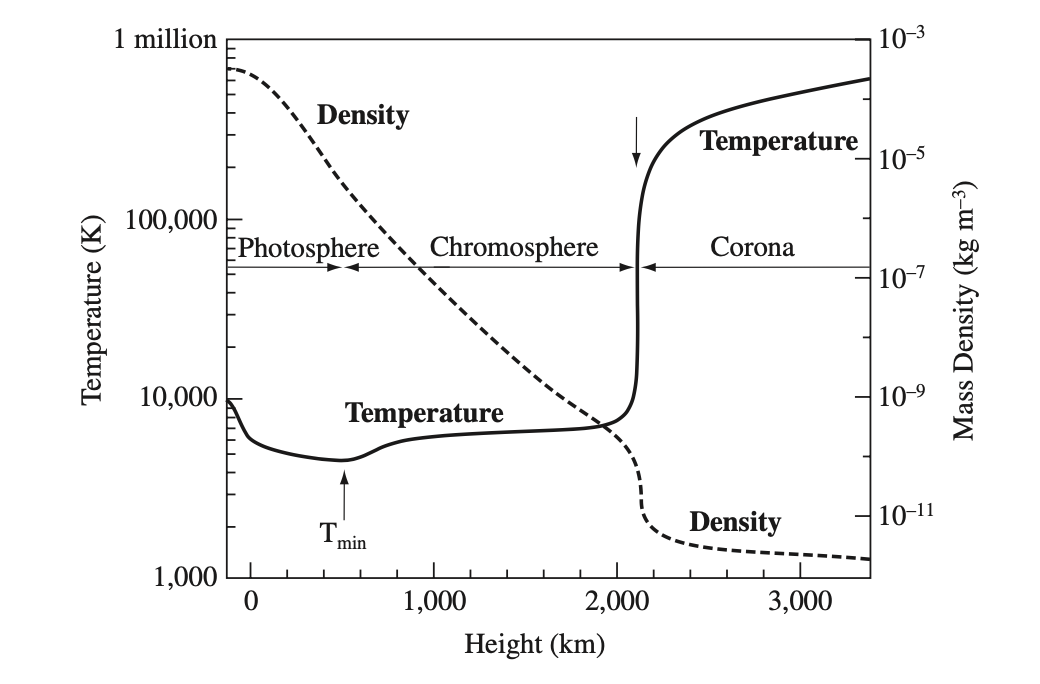
\includegraphics[width=\textwidth]{solar_profile.png}
  \caption{
    Schematic of the mean variation of the temperature and density in the solar atmosphere as a function of height.
    Figure taken from \citet{book_priest}.
  }
  \label{fig: solar_profile}
\end{figure}

The second layer is called the \emph{chromosphere}, which starts at the upper photosphere and has a fairly constant temperature with decreasing density for increasing distance from the surface. The chromosphere also contains the transition from $\beta > 1$ to $\beta < 1$, in which $\beta$ is given by
\begin{equation} \label{eq: plasma_beta}
  \beta = \frac{p_\text{gas}}{p_\text{magnetic}} = 2\mu_0 \frac{p_\text{gas}}{B^2}.
\end{equation}
Here $B$ denotes the magnetic field and $\mu_0$ the magnetic permeability in vacuum, equal to $4\pi$ in cgs units. The above quantity, called the \emph{plasma-$\beta$}, is defined as the ratio between gas pressure and magnetic pressure and is thus a measure of the relative importance of the magnetic field. For $\beta > 1$ the plasma forces dominate, which is for example the case in the solar photosphere. On the other hand, $\beta < 1$ indicates that the magnetic forces are dominant, which is the case for most of the solar corona and part of the solar chromosphere.

The chromosphere ends at the sudden rise in temperature and drop in density which is called the
\emph{transition region}. In this very narrow region of about 100 km the plasma jumps from approximately 20 000 K in the upper chromosphere to over a million K, which marks the start of the \emph{solar corona}, the third and final region in the schematic shown in Figure \ref{fig: solar_profile} and the outermost layer of the solar atmosphere. The entire corona is full of fascinating structures such as solar prominences and coronal loops, and at high altitudes the corona gives rise to the solar wind, continuously blowing plasma and particles into space.

\begin{figure}[t]
  \centering
  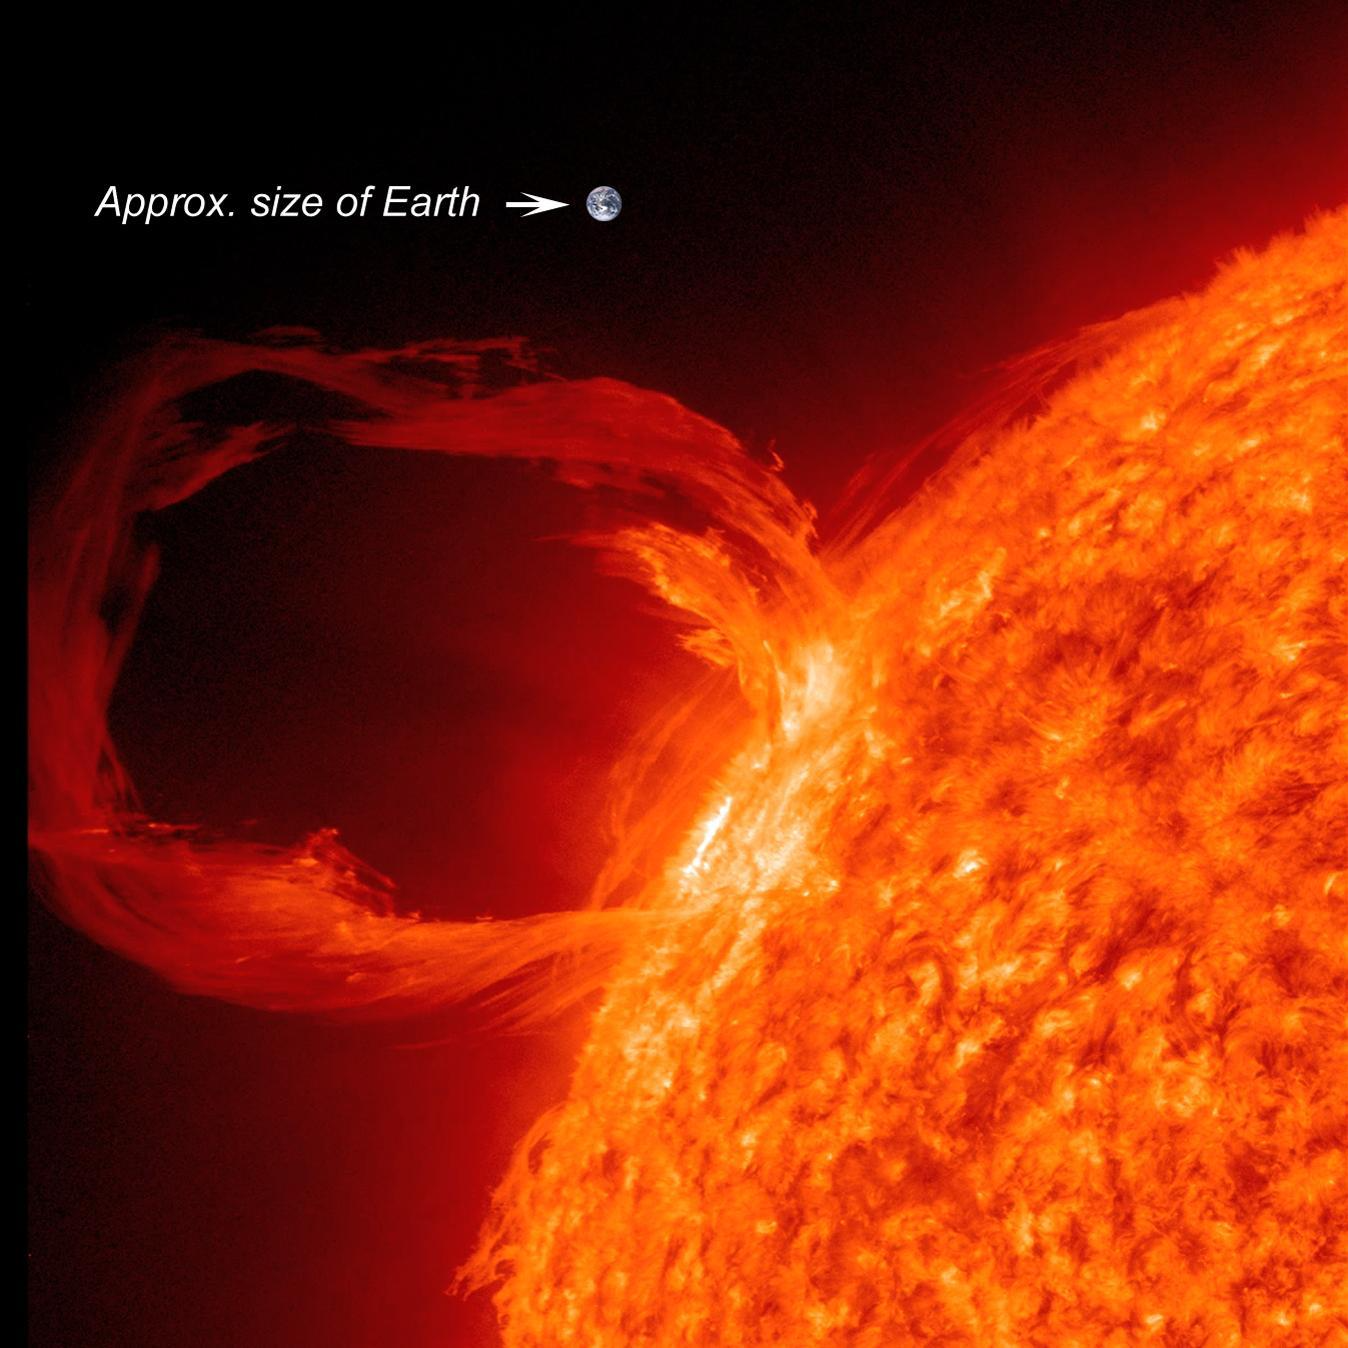
\includegraphics[width=0.6\textwidth]{solar_prominence.png}
  \caption{
    Eruptive prominence in He II at 304 {\AA} from 10 March 2010, the size of the Earth is indicated on the figure for scale. Figure from NASA/SDO/AIA.
  }
  \label{fig: solar_prominence}
\end{figure}

We will briefly discuss solar prominences in this introductory part, as they are highly relevant in the scope of Chapter \ref{ch: thermal instability}. In essence, solar prominences are large, cool, and dense structures suspended along magnetic field lines, that have their footpoints near the photosphere and extend thousands of kilometres outwards into the hot corona. They form most likely through the process of thermal instability (TI), where a runaway radiative cooling effect leads to increased energy losses through radiation, eventually leading to plasma motions that locally increase the density while energy losses drastically lower the temperature further. The resulting condensations are orders of magnitude denser and hotter than their surroundings and initial conditions, with their plasma suspended by magnetic fields high above the solar surface. This is the in-situ ``condensation'' approach to solar prominence formation, where plasma condenses in-place due to thermal instability and forms a flux rope. In the past few years variants of this process have been proposed.
The first one is an ``evaporation-condensation'' process, wherein chromospheric plasma is evaporated due to localised footpoint heating and thereby feeds material to the coronal volume, where it then condenses due to thermal instability. The steady supply of mass in this model overcomes the limitations of an in-situ TI approach, and it has been successfully employed to model solar prominences \citep{xia2016} and study the formation of coronal rain \citep{fang2013,moschou2015,xia2017}.

The second process is an injection-based model, where one can distinguish between two scenarios: ``levitation-condensation'' and ``reconnection-condensation''. The former is less dramatic than the latter, but both involve some sort of magnetic reconnection to eject plasma upwards into the solar corona instead of a steady supply through evaporation. This plasma eventually settles in already present topological dips in the field lines. The levitation mechanism mostly lifts cool, relatively static chromospheric material upwards, directly into the body of the flux rope \citep{kaneko2015,zhao2017,jenkins2021}. The reconnection mechanism on the other hand usually involves injecting material straight from the footpoints in a much more dynamic way \citep{kaneko2017}. In both scenarios the propelled material is heated to some degree due to the reconnection process, and eventually condenses through TI.
Finally, \citet{zhao2022} recently proposed a new scenario where a current sheet underneath the flux rope gives rise to magnetic islands (plasmoids), which in turn transport cool and dense chromospheric matter to the flux rope, eventually forming a prominence with coronal plasma continuously condensing through TI. Thermal instability obviously plays a critical role in all these scenarios, making a thorough understanding of TI as a whole of paramount importance.

If these giant structures become unstable they can burst outwards as an eruptive prominence. Figure \ref{fig: solar_prominence} shows such a large, eruptive prominence in He II at 304 \AA, from 10 March 2010; the Earth is superimposed for scale, making the enormous size of these structures apparent. It immediately becomes clear that waves and instabilities play a major role here. How, why and when do these structures become unstable? Can it be traced back to instabilities during their formation process? Or are there new instabilities that arise? If so, where do they come from? Furthermore, most prominences show intriguing fine structure, and it is at present still largely unknown where that originates from.

\section{The importance of instabilities}
The questions mentioned in the previous paragraph highlight the importance of wave and instability studies in all kinds of settings, not only limited to solar applications but highly relevant to a wide range of scientific disciplines. In hydrodynamics (fluids and gasses), one of the most well-known instabilities is the Kelvin-Helmholtz instability, originating from a velocity shear at the interface between two fluids (e.g. \citep{book_choudhuri}). This type of instability is commonly found in many laboratory, astrophysical and space plasmas, with some common examples being characteristic cloud formations here on Earth, ripples at the interface between solar prominences and the corona; and even near the Great Red Spot on Jupiter (see Figure \ref{fig: kh_instability}).

\begin{figure}[b]
  \centering
  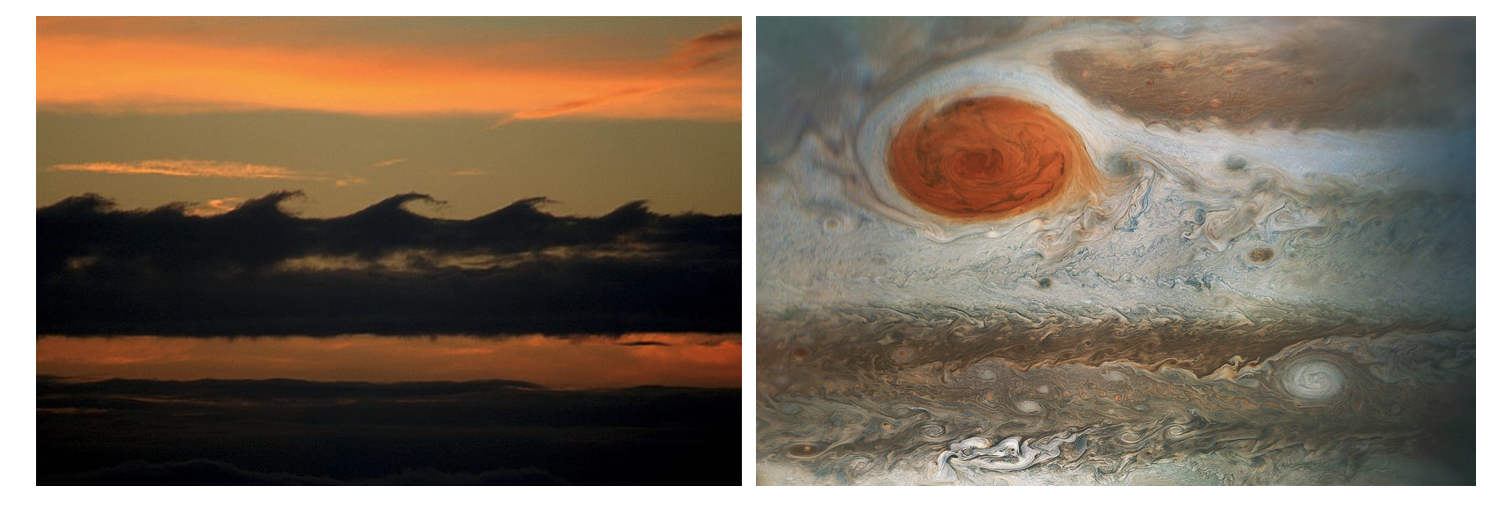
\includegraphics[width=\textwidth]{instabilities.png}
  \caption{
    Examples of Kelvin-Helmholtz instabilities in cloud formations (left) and near Jupiter's Great Red Spot (right), note the characteristic vortices for both cases. Left figure by Brocken Inaglory, right figure by NASA/JPL.
  }
  \label{fig: kh_instability}
\end{figure}

As mentioned earlier thermal instability lies at the basis of solar prominence formation, but is directly relevant to a broader astrophysical context as well. Thermal instabilities have been encountered in dense molecular clouds in the warm interstellar medium, where they can be responsible for high density filaments in star-forming regions; in galactic clusters and haloes; and even in thin discs accretion onto stellar-mass black holes where they can cause a vertical collapse of the disk. Thermal instability can occur both in hydrodynamics as in magnetohydrodynamics (plasmas), where in case of the latter the addition of a magnetic field further complicates the picture; thereby not only affecting thermal instability but all other aforementioned instabilities as well.

Magnetic fields may give rise to an even richer collection of possible instabilities in a given system. One of the more dramatic changeovers in magnetohydrodynamics lies in the introduction of magneto-rotational routes to turbulence, at play in accretion disks around black holes or in protoplanetary disks around newly formed stars \citep{balbus1991}. Not only this well-known magnetorotational instability (MRI) is important here: recent work by \citet{goedbloed2022_sari} found that a new type of mode, the Super-Alfv\'enic Rotational instability (SARI), is of essential importance for instability studies of accretion disks, and may open up novel pathways into turbulence studies.
The relevance of waves and instabilities does not limit itself to astrophysical settings, but also holds for magnetised applications accessible to laboratory experiments. This even extends to controlled nuclear fusion research, where MHD spectroscopy -- that is, classifying the various linear waves and (in)stabilities of a system -- is already the pre-eminent tool used to delimit operational windows: instabilities can strongly disrupt a given system and are to be avoided at all costs.


\section{General outline}
Due to the huge applicability and interdisciplinary importance of linear stability studies the topic is vast and numerous research has been done over the past decades. However, research in this field usually takes one of two main approaches: either direct numerical simulations are done in two or three dimensions, which is quite resource intensive and time-consuming; or a theoretical approach is considered in which the required dispersion relation makes it necessary to use (greatly) simplifying assumptions due to the complexity of the problem at hand. In this thesis we plan to take a different approach to waves and instabilities, and tackle (thermal) instabilities from a spectroscopic viewpoint. We therefore take a stepwise approach and formulate the following:
\begin{enumerate}
  \item[i)] How do linear waves trigger or evolve into nonlinear thermal instability for local coronal volumes?
  \item[ii)] In the nonlinear regime, is there a link between thermal instability and fine structure?
  \item[iii)] Moving away from simplified setups, what does the spectrum of a realistic solar atmosphere look like?
  \item[iv)] What role do thermal instabilities have in this?
\end{enumerate}

These can be regarded as the ``science questions'' we want to look at in this thesis, with point iii) and iv)  being quite challenging. In order to lay a solid foundation we dedicate Chapter \ref{ch: spectroscopy} to a thorough introduction to MHD spectroscopy, paying special attention to the non-adiabatic terms.

Chapter \ref{ch: thermal instability} builds further upon this, where a combined numerical and theoretical approach in a simplified uniform setup allows us to derive eigenfunctions for slow MHD modes, which can then be excited in a numerical domain with solar coronal conditions. We can make sure that the thermal mode is unstable, and we can take a close-up look at the dynamical and temporal evolution of the system as a whole. This gives us a first answer to points i) and ii).

In order to look at point iii) we need to move away from ``simple'' setups, which implies that problems can no longer be treated analytically. Therefore, in Chapter \ref{ch: legolas} we lay the foundations for the development of a brand new numerical tool, {\legolas}, which will allow us to do MHD spectroscopy of one-dimensional equilibria with a plethora of physical effects, for a general configuration that achieves force and thermodynamic balance. We introduce the weak Galerkin form of the linearised and Fourier-analysed MHD equations, which in turn transforms the set of equations in a generalised eigenvalue problem that can be solved using various linear algebra routines. This results in a complete set of eigenvalues and eigenfunctions for a given state, allowing us to probe the various waves and (in)stabilities at high resolutions.

In Chapter \ref{ch: legolas_applications} we test {\legolas} against a whole range of well-established results, from p and g modes in magnetised, stratified atmospheres, to modes relevant for coronal loop seismology, thermal instabilities, and instability studies of astrophysical jet flows. We show an excellent correspondence with known results, thereby thoroughly testing the implementation of our new code.

Finally, with {\legolas} we are in a place to answer points iii) and iv), and hence look at a realistic, empirical solar atmosphere model in Chapter \ref{ch: solar_atmosphere} and calculate the full eigenvalue spectrum for different chromospheric and coronal regions. This yields new insights in the behaviour of the thermal and slow continua, as well as in the thermal stability of these kinds of configurations.




\cleardoublepage
